
\section{Experiment}
\label{experiment}



\begin{table*}
\small
    \centering
    \renewcommand{\tabcolsep}{3.0pt}
    \renewcommand{\arraystretch}{1.0}
    \begin{tabular}{ccccccccc}
    \hline
        \multirow{2}{*}{Methods} & \multicolumn{3}{c}{Auto Evaluation} & \multicolumn{5}{c}{Human Evaluation} \\
        \cmidrule[\cmidrulewidth](r{0.5em}){2-4}  \cmidrule[\cmidrulewidth](r{0.5em}){5-9}
        & Word Num. & $CR.\downarrow$  & ${Ent-2}\uparrow$ &$PCo.\downarrow$ &$PCoh.\downarrow$ &$Rel.\downarrow$ & $Int.\downarrow$ &$Ecoh.\downarrow$ \\
        
        \hline
        Llama3-70B-Instruct~\cite{llama3} &612.65  &6.78   &9.25 &3.77  &3.81  &3.58  &3.96  &3.72  \\
        Qwen1.5-72B-Chat~\cite{bai2023qwen} &495.70   &0.66  &9.06 &4.77  &4.80  &4.58  &4.96  &4.72   \\
        \hline
        Re$^3$~\cite{Re3} &3802.15 &0.77 &11.56 &2.73  &2.53  &2.96  &2.56  &2.83    \\
        DOC~\cite{DOC} &3904.90  &1.21 &11.55 &2.58  &2.43  &2.63  &2.34  &2.56  \\
        \rowcolor{mycyan}[1.2ex][1.5ex] \textbf{Ours (Qwen1.5-72B-Chat)} &\textbf{7113.75} &\textbf{0.56} &\textbf{12.29} &\textbf{1.15}  &\textbf{1.44}  &\textbf{1.26}  &\textbf{1.77} & \textbf{1.16}  \\
        \hline
    \end{tabular}
    \caption{Comparison with LLMs and SOTA baselines. We use the same premises as DOC~\citet{DOC}.}
    \label{tab:human_eval}
\end{table*}


\begin{table*}
\small
    \centering
    \renewcommand{\tabcolsep}{3.0pt}
    \renewcommand{\arraystretch}{1.0}
    \begin{tabular}{ccccccccc}
    \hline
        \multirow{2}{*}{Methods} & \multicolumn{3}{c}{Auto Evaluation} & \multicolumn{5}{c}{Human Evaluation} \\
        \cmidrule[\cmidrulewidth](r{0.5em}){2-4}  \cmidrule[\cmidrulewidth](r{0.5em}){5-9}
        & Word Num. & $CR.\downarrow$  & ${Ent-2}\uparrow$ &$PCo.\downarrow$ &$PCoh.\downarrow$ &$Rel.\downarrow$ & $Int.\downarrow$ &$Ecoh.\downarrow$ \\
        
        \hline
        w/o MEM  &6511.10  &4.52    &10.00 &1.88   &2.24  &1.97  &1.96   &2.22  \\
        w/o DHO &1471.90   &0.65  &11.50 &2.92  &2.36  &2.86  &2.88  &2.46   \\
        \rowcolor{mycyan}[1.2ex][1.5ex] \textbf{Ours (Qwen1.5-72B-Chat)} &\textbf{7113.75} &\textbf{0.56} &\textbf{12.29} &\textbf{1.20}  &\textbf{1.40}  &\textbf{1.17 }  &\textbf{1.62} & \textbf{1.32}  \\
        \hline
    \end{tabular}
    \caption{Ablation study of different modules.}
    \label{tab:Ablation}
    % \vspace{-6pt}
\end{table*}


\textbf{Implementation details. }
\wqyr{\methodname~\footnote{The implementation are available at \url{https://github.com/Qianyue-Wang/DOME}}contains DHO and MEM. In DHO, every rough outline is expanded into 3 detailed outlines which means the $M$ mentioned in Section \ref{sec:dho} is set to 3. The embedding model we applied is bge-large-en-v1.5~\cite{chen2024bge}. In MEM, \wqyr{we apply cosine similarity~\cite{lahitani2016cosine} and set the filter threshold to 0.75 to implement the entity-based query.}}
Besides, we switch off the default historical content input of LLM where MEM is applied. The temperature of LLM is set to 0.5 and the max token of LLM is 1000 while other parameters are kept by default. All the experiments are conducted on 2$\times$A800 GPU with CUDA version 11.3.


\textbf{Datasets and baselines. }\wqyr{Following the settings of DOC~\cite{DOC}, we use its story premises\footnote{All the datasets are available at \url{https://github.com/Qianyue-Wang/DOME_dataset}} as the input and generate 20 long stories for evaluation. The details of the dataset are in Appendix~\ref{sup:Datasets Detsils}.}{We use Qwen1.5-72B-chat~\cite{bai2023qwen} for long-form story generation as it has considerable performance~\cite{chiang2024chatbot} and can be deployed locally. We compare \methodname~with two types of methods. The first is prompting LLM to generate stories as long as possible with input. The second are the state-of-the-art (SOTA) methods including DOC~\cite{DOC} and Re$^3$~\cite{Re3}. To validate the scalability of \methodname, we report the improvement When applying \methodname~ on Llama-3-70b-Instruct~\cite{llama3} and Yi1.5-34B-chat~\cite{young2024yi}.
 }

\textbf{Metrics. }
\wqyr{Since the content repetition is an important aspect reflecting the quality of stories in terms of coherence~\cite{Re3}, We apply the auto evaluation metrics including n-gram entropy~\cite{zhang2018generating} and set $n=2$ ($Ent$-2) to evaluate the degree of content repetition by measuring the diversity of vocabulary. Besides, we apply our proposed conflict rate ($CR.$) to evaluate the contextual consistency of the generated stores.} \par
\wqyr{To evaluate the alignment of the stories with human preferences in terms of contextual consistency and coherence and other basic story quality, we further conduct a human evaluation to evaluate the story quality of plot completeness, coherence, relevance, interest level, and expression coherence.} 
We compare all methods according to each indicator and calculate their average rank. The description of every metric is as follows: 
    1) Plot Completeness ($PCo.$): the extent to which the generated story covers all the stages mentioned in the story theory.
    2)  Plot Coherence ($PCoh.$): the fluency of the development of the generated story.
    3)  Relevance ($Rel.$): the consistency between the generated story and the input premise. \wqyr{It demonstrates the actual usability of the method.}
    4)  Interesting ($Int.$): the reading interest to the user. \wqyr{Since the reading interest can reflect peoples' preferences on the completeness and coherence of stories \cite{wang-etal-2023-improving-pacing}.}
    5)  Expression Coherence ($ECoh.$): the contextual consistency of the story.
More details of human devaluation are shown in Appendix~\ref{sup:human evaluate}.

\subsection{Comparison experiments}

\textbf{\methodname~is consistently better in auto evaluation.} From Table \ref{tab:human_eval}, the proposed \methodname~achieves superior performance in both $CR.$ and $Ent$-2. It also generates the longest content.
Specifically, \methodname~surpasses the LLM baseline, Qwen1.5-72B-Chat, by 35.7\% in $Ent$-2 and reduce the $CR.$ by 15.2\%. Additionally, \methodname~outperforms the Re$^3$ by 6.3\% in $Ent$-2 and reduces the $CR.$ by 27.3\%. The results indicate that our \methodname~delivers diverse content with fewer conflicts. We attribute the improvement to the following facts. Firstly, our TKG is capable of fine-grained modeling of generated stories. It provides accurate relevant content through semantic filtering during the generation stage, which ensures consistency and reduces contextual conflicts in the generated content. Besides, Our DHO dynamically adjusts the detailed outlines during the story generation process, thereby increasing the space for plot development and enhancing content diversity.

\textbf{\methodname~is consistently better in human evaluation.}We conduct a human evaluation to assess how well \methodname~aligns with human preferences. In Table \ref{tab:human_eval}, our \methodname~ranks first across all five metrics. The results demonstrate that MEM can provide relevant content during the generation stage, reducing the conflict due to the unclear memory of LLM itself~\cite{zhang2023siren} and thus ensuring contextual consistency and enhancing relevance and expression coherence. Furthermore, our DHO dynamically generates detailed outlines based on the development of the storyline, adapting to the uncertainty in generation and achieving improved fluency. Additionally, our novel-writing mechanism encourages large language models to create stories like writing a complete novel. This approach ensures the plot's completeness and to some extent, introduces fluctuations that capture and maintain reader interest.



\subsection{Ablation studies}

\textbf{Effectiveness of DHO.}\wqyr{We remove the DHO so that the outline is fixed and consistent with the input storyline.} As shown in Table \ref{tab:Ablation}, this variant exhibits higher content conflicts and reduced content \wqyr{variety}. Additionally, it ranks lowest across all human evaluation metrics. It supports the notion that dynamic adjustment of the detailed outline helps to control content generation, thereby ensuring plot coherence. Furthermore, the application of novel writing theory enhances plot completeness and thus improves the reading interest, \wqyr{this is because a complete story encourages the reader to read to the end.} See the example of DHO in Appendix~\ref{sup:dho example}.



\textbf{Effectiveness of MEM.}
Similarly, we remove the MEM to eliminate the knowledge graph for reference and resort to the multi-round chatting capability of LLM to generate content. Limited by computing cost, we set the maximum chat rounds to 2. \wqyr{As shown in Table \ref{tab:Ablation}}, the conflict rate significantly increases from 0.56 to 4.52 and $Ent$-2 reduces from 12.29 to 10.00 without MEM. Additionally, all human evaluation metrics deteriorate to varying degrees. These results indicate that MEM ensures contextual coherence by providing relevant content during generation, which also improves plot coherence and alignment with human preferences. See the example of MEM in Appendix~\ref{sup:mem example}.

\begin{figure}[t]
\centering
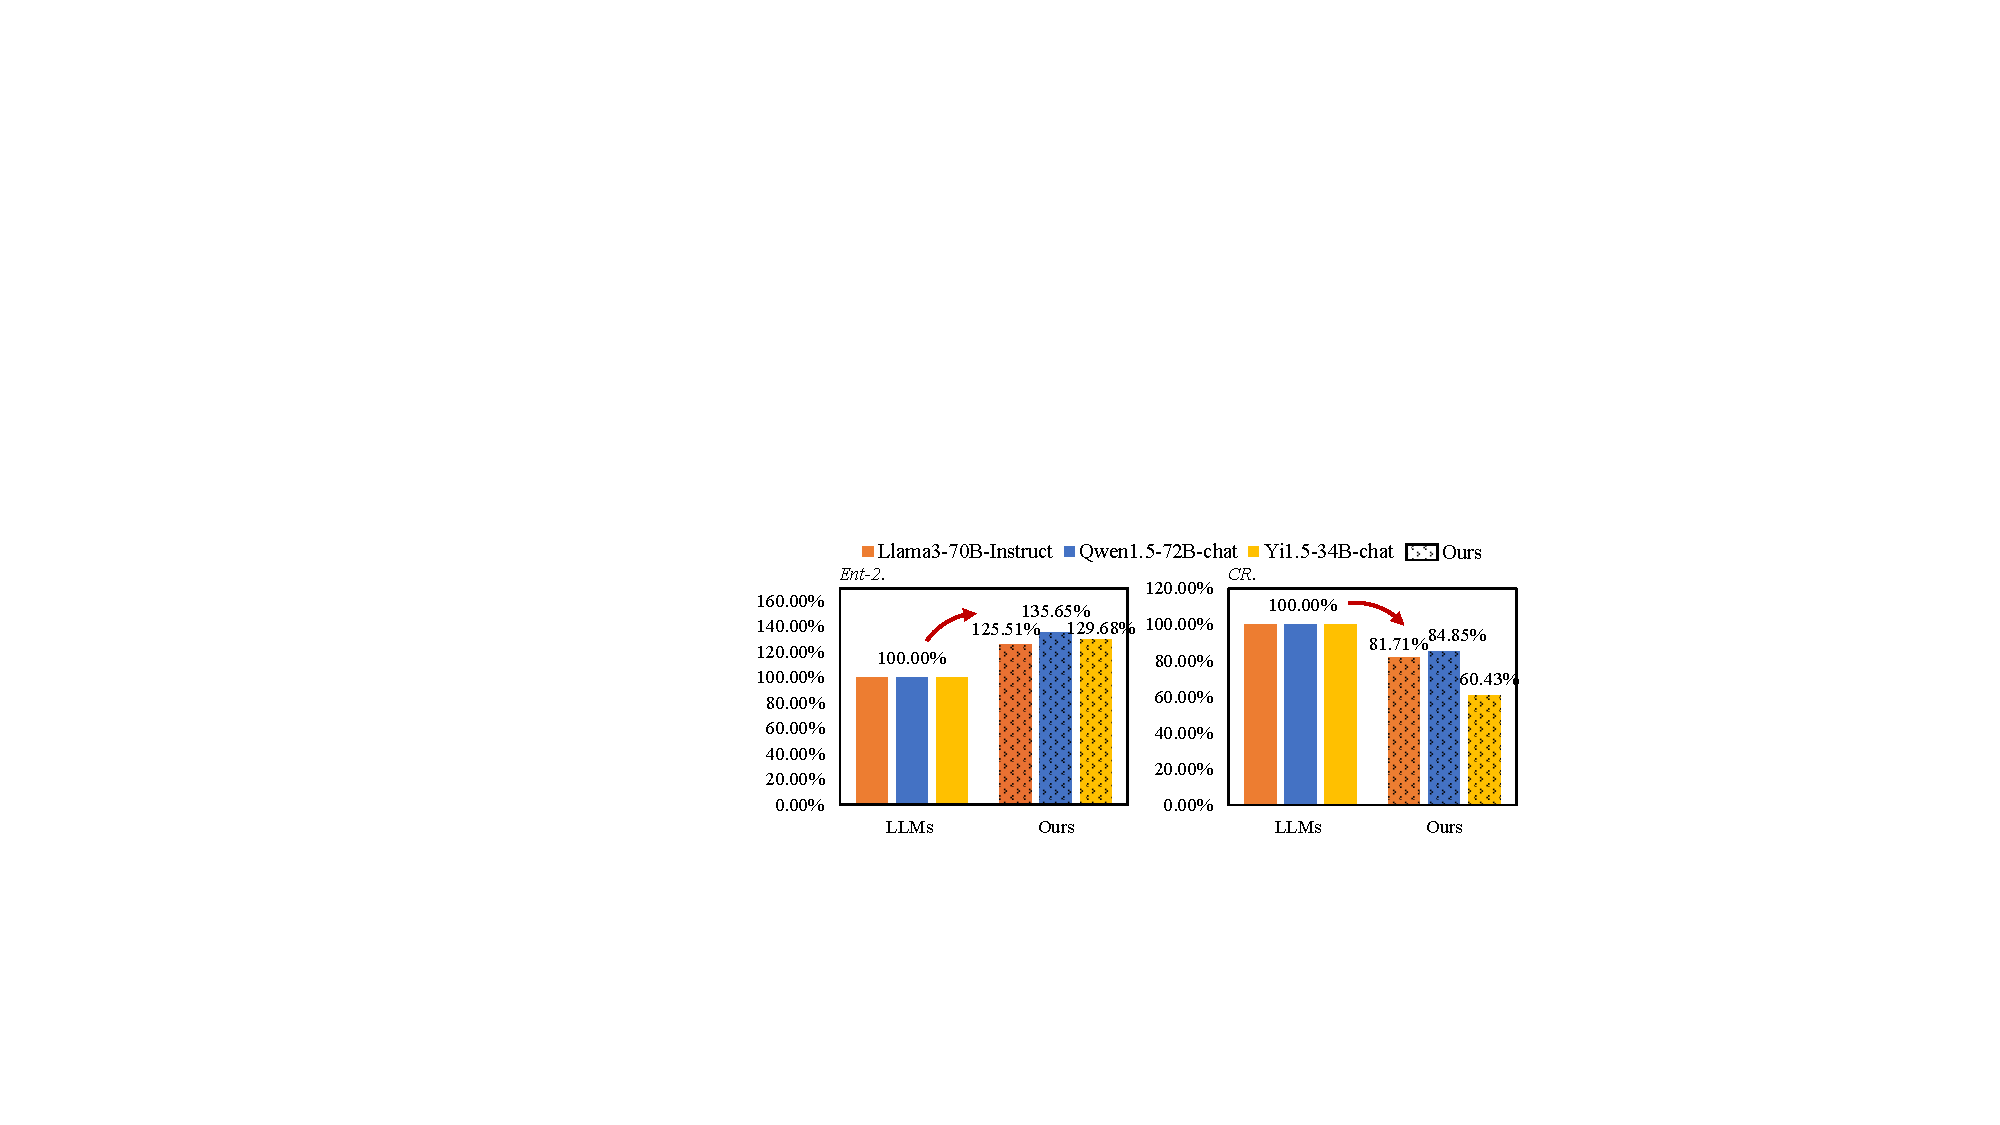
\includegraphics[width=1.0\linewidth]{images/eval-bar2.pdf}

    \caption{
    Scalability results of applying~\methodname~on different LLMs. Left: the increase rates of $Ent$-2 metric. Right: the decrease rates of $CR.$ metric.
    }  
    \label{fig:exp3}
\vspace{-6pt}
\end{figure}
\subsection{The Scalability of \methodname}

\wqyr{To demonstrate the applicability of \methodname~on different LLMs, we apply our method to  Yi1.5-34B-chat, Llama3-70B-Instruct and Qwen1.5-72B-chat. As illustrated in Fig.~\ref{fig:exp3}, \methodname~significantly reduces conflicts and enhances content diversity on all LLMs with different parameter scales. Specifically, \methodname~reduce the $CR.$ by more than 18\% on Llama3-70B-Instruct. It also improves the $Ent$-2 by more than 29\% on Yi1.5-34B-chat. This scalability is due to the straightforward and easy-to-follow prompts in our \methodname, making it easy to be adaptable across different LLMs. }


\begin{table}[t]
\small
    \centering
    \renewcommand{\tabcolsep}{1pt}
    \renewcommand{\arraystretch}{1.2}
    \begin{tabular}{ccccccccc}
    \hline
        LLM (w \methodname) & Nodes	&Relations	&Quadruples &API calls\\ \hline
        Yi1.5-34B-chat & 691.3	&328.45 &354.55&16\\ 
        Llama3-70B-instruct& 844.6	& 345.65& 434.0&16\\
        Qwen1.5-72B-chat & 791.35	&258.23	&404.85 &16\\
        \hline
    \end{tabular}
    \caption{\wqyr{The computation and storage cost of \methodname. Notable the API calls means the average number of API calls for KG construction.}}
    \label{tab: storage cost}
    \vspace{-6pt}
\end{table}

\subsection{\wqyr{Computation and storage cost of \methodname}}
\wqyr{We report the computation and storage cost for constructing the knowledge graph dynamically, as shown in Table \ref{tab: storage cost}. With acceptable additional computation and storage overhead, the proposed method improves the quality of generating long-form stories. Specifically, as shown in Tables \ref{tab:human_eval} and \ref{tab: storage cost}, the proposed DOME only adds 791 nodes of storage overhead and 16 LLM API calls to construct the KG dynamically, but it outperforms the SOTA methods in all performance metrics. This is because the structured storage of KG and the access advantages of KG facilitate LLM in achieving accurate and concise relevant memory and reducing context inconsistency.}
